\documentclass{beamer}
\usepackage[english]{babel}
\usepackage{tikz}
\usetikzlibrary{backgrounds,positioning,fit}

\begin{document}

\begin{frame}
\frametitle{My slide}

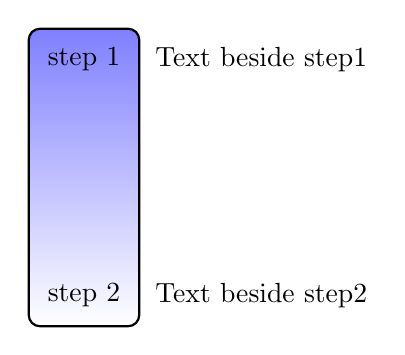
\begin{tikzpicture}
\node (step1) at (0, 0) {step 1};
\node (step2) at (0, -3) {step 2};
\begin{pgfonlayer}{background}
\node [fit = (step1) (step2),framed, thick, draw=black, top color=blue!50, rounded corners] {};
\end{pgfonlayer}
\node [right=0.2cm of step1, anchor = west] {Text beside step1};
\node [right=0.2cm of step2, anchor = west] {Text beside step2};
\end{tikzpicture}
\end{frame}

\end{document}
